% \section{TC $G$-Pooling: Group-Invariant Pooling with the Triple Correlation}
\section{The $G$-Triple-Correlation Layer for Robust $G$-Invariance}\label{sec:g-tc}

We propose a $G$-Invariant layer designed for $G$-CNNs that is \textit{complete}\textemdash that is, it preserves all information about the input signal except for the group action. Our approach leverages the theory of the triple correlation on groups~\cite{kakarala1992triple} and applies it to the design of robust neural network architectures. Its theoretical foundations in signal processing and invariant theory allows us to generally define the unique $G$-invariant maps of lowest polynomial order that are complete, hence providing a general framework for selective, robust $G$-invariance in $G$-CNNs \cite{sturmfels2008algorithms}.

 % Our pooling operation is typically performed after the $G$-convolution, so that we restrict its definition to signals defined over a group $G$.
%However, we note that the definition exists for any signal defined over a domain that is homogeneous for a group.

\subsection{The $G$-Triple-Correlation Layer}

% The \textit{triple correlation} (TC) on group $G$ is defined:

% \begin{equation}
%     \int_{-\infty}^{\infty}f(x)f(\mathcal{L}_{g_1} x) f(\mathcal{L}_{g_2} x) dx
%     \end{equation}

The \textit{$G$-Triple-Correlation} ($G$-TC) on a real signal $\Theta: G \rightarrow \mathbb{R}$ is the integral of the signal multiplied by two independently transformed copies of it~\cite{kakarala1992triple}:
% \begin{equation}
%     \tau_f(g_1, g_2) = \int_{u \in \domain} f(u) f(T_{g_1}(u)) f(T_{g_2}(u)) du.
% \end{equation}
% \begin{equation}
%     \tau_f(g_1, g_2)
%         =
%         \int_{g \in G}
%         f(T_g(u_0))
%         f\left(T_{g g_1}(u_0)\right) f\left(T_{g g_2}(u_0)\right)
%         dg .
% \end{equation}
\begin{equation}
    \tau_\Theta(g_1, g_2)
        = \int_{g \in G} \Theta(g) \Theta\left(g g_1\right) \Theta\left(g g_2\right)dg .
\end{equation}
This definition holds for any locally compact group $G$ on which we can define the Haar measure $dg$ used for integration purposes~\cite{KakaralaTriple}. This definition above is applicable to the $G$-CNNs where $\Theta$ is a collection of scalar signals over the group. We show in Appendix~\ref{app:steerable} that we can extend the definition to steerable $G$-CNNs where $\Theta$ can be an arbitrary field~\cite{cohen2016steerable}.

In the equation above, the $G$-TC is computed for a pair of group elements $g_1, g_2$. In practice, we sweep over all pairs in the group. Appendix \ref{app:tc-examples} illustrates the triple correlation on three concrete groups. Importantly, the $G$-triple-correlation is invariant to the action of the group $G$ on the signal $\Theta$~\cite{KakaralaTriple}, as shown below.
\begin{proposition}Consider a signal $\Theta: G \mapsto \mathbb{R}^c$. The $G$-Triple-Correlation $\tau$ is $G$-invariant:
\begin{equation}
    \tau_{L_g[\Theta]} = \tau_{\Theta}, \quad \text{for all $g \in G$,}
\end{equation}
where $L_g$ denotes an action of a transformation $g$ on the signal $\Theta$.
\end{proposition}

The proof is recalled in Appendix~\ref{sec:g-tc-invariance}. We propose to achieve $G$-invariance in a $G$-CNN by applying the $G$-Triple-Correlation ($G$-TC) to the output $\Theta$ of a $G$-convolutional layer. Specifically, we apply the $G$-TC to each real scalar valued signal $\Theta_k$ that comes from the $G$-convolution of filter $\phi_k$, for $k \in \{1, ..., K\}$. We only omit the subscript $k$ for clarity of notations. In practice, we will use the triple correlation on discretized groups, where the integral is replaced with a summation:
% In practice, we will use the triple correlation on the output of the $G$-convolutional layers, which are functions defined over a discretized group. In this context, the triple correlation is defined as:
% \begin{equation}\label{eq:tcpool}
%     \tau_\Theta(g_1, g_2)= \sum_{g \in G}\Theta(g) \Theta\left(g g_1\right) \Theta\left(g g_2\right),
% \end{equation}
% \begin{equation}
%     \Theta_{\mathrm{TCPOOL}}(i, j) = \sum_x f(x) f(x)_i  f(x)_j
%     \end{equation}

% \begin{equation}
%     \Theta_{\mathrm{TCPOOL}}(i, j)_k = \sum_x \Theta_k(x) \Theta_k(g_i) \Theta_k(g_j)
%     \end{equation}
% TODO (?): What is the impact of the discretization if the group cannot be perfectly discretized (e.g. SO(3))?


% \textbf{Version 1
% }
% We define the TC $G$-Pooling layer:

% \begin{equation}
%     \sum_x f(x)f(\mathcal{L}_{g_1} x) f(\mathcal{L}_{g_2} x)
%     \end{equation}


% \textbf{Version 2}

\begin{equation}
    T_\Theta(g_1, g_2)= \sum_{g \in G} \Theta(g) \Theta(gg_1) \Theta(gg_2),
    \end{equation}
for $\Theta$ a scalar valued function defined over $G$.
%The output of a $G$-conv layer computed for group action $g$ and filter $k$ is written $\Theta_k$ which is a function of a discretized group $G$. The TC layer is defined:
While it seems that the layer computes $T_\Theta(g_1, g_2)$ for all pairs of group elements $(g_1, g_2)$, we note that the real scalars $\Theta(gg_1)$ and $\Theta(gg_2)$ commute so that only half of the pairs are required. We will see that we can reduce the number of computations further when the group $G$ possesses additional properties such as commutativity.

% Specifically, the TC $G$-pooling proposed here is the unique complete $G$-pooling method \cite{otherpaper}.

% \begin{figure}
%     \centering
%     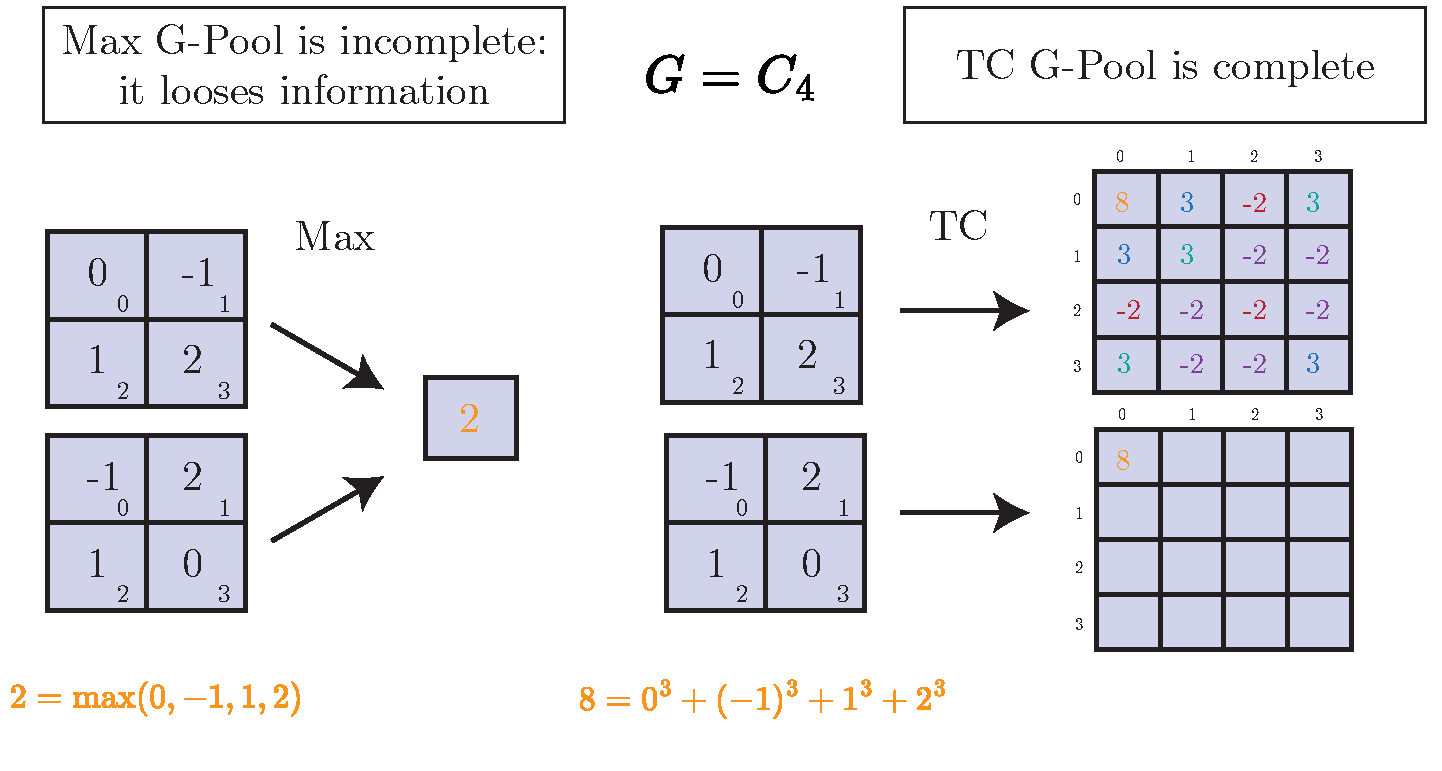
\includegraphics[width=0.7\textwidth]{figs/background-poolings-c4.pdf}
%     \caption{[Figure summarizing our method]}
%     \label{fig:background-poolings-c4}
% \end{figure}

We note that the triple correlation is the spatial dual of the \textit{bispectrum}, which has demonstrated robustness properties in the context of deep learning with bispectral neural networks \cite{sanborn2023bispectral}. The goal of bispectral neural networks is to learn an unknown group $G$ from data. The bispectral layer proposed in \cite{sanborn2023bispectral} assumes an MLP architecture. Our work is the first to generalize the use of bispectral invariants to convolutional networks. Here, we assume that the group $G$ is known in advance, and exploit the theoretical properties of the triple correlation to achieve robust invariance. One path for future extension may be to combine our approach with the learning approach of \cite{sanborn2023bispectral}, to parameterize and learn the group $G$ that defines a $G$-Equivariant and $G$-Invariant layer.

\subsection{Selective Invariance through Completeness}

We show here that the proposed $G$-triple-correlation is guaranteed to preserve all information aside from any equivariant component due to the group action on the input domain. This crucial property distinguishes our proposed layer from standard $G$-Pooling methods, which collapse signals and lose crucial information about the input (Figure \ref{fig:overview-cnn-c4}). In contrast with standard, excessively invariant $G$-pooling methods, we show here that our $G$-TC layer is instead \textit{selectively} $G$-invariant thanks to its \textit{completeness} property \cite{yellott1992uniqueness, kakarala1993group, kakarala2012bispectrum}, defined here:

% The triple correlation is said to be \textit{complete}, in a sense made precise by the following proposition~ \cite{yellott1992uniqueness, kakarala1993group, kakarala2012bispectrum}.

\begin{proposition}
    Every integrable function with compact support $G$ is completely identified\textemdash up to group action\textemdash by its $G$-triple-correlation. We say that the $G$-triple-correlation is complete.
\end{proposition}

Mathematically, an operator $\mathcal{T}$ is complete for a group action $L$ if the following holds: for every pair of signals $\Theta_1$ and $\Theta_2$, if $\mathcal{T}(\Theta_1) = \mathcal{T}(\Theta_2)$ then the signals are equal up to the group action, that is: there exists a group element $h$ such that $\Theta_2 = L_h[\Theta_1]$.

The proof of the completeness of the $G$-triple-correlation is only valid under a precise set of assumptions~\cite{kakarala1992triple} (Theorem 2). As we seek to integrate the $G$-triple-correlation to enhance robustness in neural networks, we investigate here the scope of these assumptions. First, the assumptions are not restrictive on the type of groups $G$ that can be used. Indeed, the proof only requires the groups to be Tatsuuma duality groups and the groups of interest in this paper meet this condition. This includes all locally compact commutative groups, all compact groups including the groups of rotations, the special orthogonal groups $SO(n)$, and groups of translations and rotations, the special euclidean groups $SE(n)$. Second, the assumptions are not restrictive on the types of signals. Indeed, the signal only needs to be such that any of its Fourier transform coefficients are invertible. For example, when the Fourier transform coefficients are scalar values, this means that we require these scalars to be non-zero. In practical applications on real image data with noise, there is a probability 0 that the Fourier transform coefficients of the input signal will be exactly 0 (scalar case) or non-invertible (matrix case). This is because the group of invertible matrices is dense in the space of matrices. Therefore, this condition is also verified in the applications of interest and more generally we expect the property of completeness of our $G$-TC layer to hold in practical neural network applications.

\subsection{Uniqueness}

The above two subsections prove that our $G$-Triple Correlation layer is selectively $G$-invariant. Here, we note that our proposed layer is the lowest-degree polynomial layer that can achieve this goal. In invariant theory, it is observed that the $G$-Triple Correlation is the \textit{only} third-order polynomial invariant (up to change of basis) \cite{sturmfels2008algorithms}. Moreover, it is the lowest-degree polynomial invariant that is also complete. It thus provides a unique and minimal-complexity solution to the problem of robust invariance within this function class.
 % Additionally, we can show that the TC $G$-Pooling is the only $G$-pooling that is indeed complete.

\subsection{Computational Complexity}

The $G$-Triple Correlation enjoys some symmetries that we can leverage to avoid computing it for each pair of group elements (which would represent $|G|^2$ computations), hence making the feedforward pass more efficient. We summarize these symmetries here.
\begin{proposition}
Consider two transformations $g_1, g_2 \in G$. The $G$-Triple Correlation of a real signal $\Theta$ has the following symmetry:
\begin{align*}
     T_\Theta(g_1, g_2) &= T_\Theta(g_2, g_1).
\end{align*}
If $G$ is commutative, the $G$-Triple Correlation of a real signal has the following additional symmetries:
\begin{align*}
     T_\Theta(g_1, g_2)
     = T_\Theta(g^{-1}_1, g_2g^{-1}_1)
     = T_\Theta(g_2g^{-1}_1, g^{-1}_1)
     = T_\Theta(g^{-1}_2, g_1g^{-1}_2)
     = T_\Theta(g_1g^{-1}_2, g^{-1}_2).
\end{align*}
\end{proposition}


The proofs are given in \cite{nikias1993signal} for the group of translations. We extend them to any locally compact group $G$ in Appendix~\ref{app:symmetries}. In practice, these symmetries mean that even if there are theoretically $|G|^2$ computations, this number immediately reduces to $\frac{|G|(|G|+1)}{2}$ and further reduces if the group $G$ of interest is commutative. In addition, more subtle symmetries can be exploited to reduce the computational cost to linear $|G|+1$ for the case of one-dimensional cyclic groups \cite{kondor2008thesis} by considering the spectral dual of the $G$-TC: the bispectrum. We provide a computational approach to extend this reduction to more general, non-commutative groups in Appendix~\ref{app:reduction}. The theory supporting our approach has yet to be extended to this general case. Thus, there is an opportunity for new theoretical work that further increases the computational efficiency of the $G$-Triple-Correlation.

% The triple correlation is a \textit{complete invariant} for [...].

% The work of Yellott and Iversons \cite{yellott1992uniqueness} established that every integrable function with compact support is completely identified\textemdash up to translation\textemdash by its three-point autocorrelation and thus its bispectrum (Appendix \ref{appendix:autocorrelation}). Later work of Kakarala tied the bispectrum to the more general formulation of Fourier analysis and thus defined it for all compact groups \cite{kakarala1993group, kakarala2012bispectrum}. Kakarala went on to prove that it is complete \cite{kakarala2009completeness} in both commutative and non-commutative formulations (Appendix \ref{appendix:completeness}).
